\section{Dettagli implementativi}

% Just report interesting / non-trivial / non-obvious implementation details.

% This section is expected to be short in case some documentation (e.g. Javadoc or Swagger Spec) has been produced for the software artefacts.
% %
% This this case, the produced documentation should be referenced here.

\subsection{Documentazione}

%
%
%
\subsubsection{Swagger}
Swagger è un insieme di strumenti open source per progettare, creare, documentare e consumare servizi web RESTful, attraverso la specifica \emph{Open API}.
%
L'obiettivo principale di Swagger è semplificare e standardizzare il processo di sviluppo e integrazione di API, fornendo una documentazione interattiva e uno strumento per testare direttamente le API.

Le caratteristiche chiave di Swagger includono:

\begin{itemize}
    \item Definizione della API: Swagger utilizza il formato YAML o JSON per definire la struttura e i dettagli di un'API RESTful, specificando risorse, operazioni, parametri, tipi di dati, e altro ancora.
    
    \item Interfaccia Utente Interattiva: Genera automaticamente un'interfaccia utente interattiva (Swagger UI) basata sulla definizione dell'API. Questa interfaccia consente agli sviluppatori di esplorare e testare le API direttamente dal browser.

    \item Standardizzazione e Conformità: Swagger promuove la standardizzazione nelle API RESTful, migliorando la coerenza e la comprensione tra sviluppatori e team di sviluppo
\end{itemize}

%
%
%
\paragraph{Utilizzo}

Con Swagger, è stato possibile creare documentazione dettagliata delle API, specificando dettagli come gli endpoint, i parametri, i tipi di dati, le risposte possibili e persino esempi di richieste e risposte.

Inizialmente, lo strumento è stato utilizzato per realizzare il design del sistema, permettendo di documentare ciò che si sarebbe dovuto implementare.
%
I cicli iterativi di raffinamento hanno permesso di convergere all'attuale stato dell'\emph{API}.

La documentazione delle API del progetto è consultabile sulle Github Pages:
\url{https://zucchero-sintattico.github.io/piperchat/api/rest/}

%
%
%
\subsubsection{AsyncApi}

AsyncAPI è uno standard di specifica per la progettazione di API asincrone.
%
Simile a come OpenAPI è utilizzato per definire e documentare API sincrone, AsyncAPI è progettato specificamente per gestire le comunicazioni asincrone, come quelle basate su messaggi o eventi.

Le principali caratteristiche di AsyncAPI includono:

\begin{itemize}
    \item Comunicazioni Asincrone: AsyncAPI è progettato per modellare API che coinvolgono comunicazioni asincrone, dove la richiesta e la risposta non sono sincronizzate nel tempo.

    \item Documentazione Dettagliata: Come OpenAPI per API sincrone, AsyncAPI fornisce una specifica dettagliata per documentare aspetti come endpoint, messaggi, schemi dei dati, protocolli di trasporto e altri dettagli relativi alla comunicazione asincrona.

    \item Supporto per Protocolli Comuni: AsyncAPI supporta una varietà di protocolli comuni per la comunicazione asincrona, come MQTT, AMQP e WebSocket. Ciò consente una flessibilità nella progettazione delle API a seconda delle esigenze specifiche del progetto.
\end{itemize}

%
%
%
\paragraph{Utilizzo}

AsyncAPI è stato utilizzato come strumento di supporto e di documentazione di tutte le tipologie di messaggi rappresentanti gli eventi che vengono scambiati tramite il broker all'interno dell'architettura a microservizi.

La documentazione delle API per i messaggi \textit{infra-servizi} è consultabile sulle Github Pages:
\url{https://zucchero-sintattico.github.io/piperchat/api/infra-service/}

Inoltre, la tecnologia è stata sfruttata anche per la documentazione dei messaggi \textit{inviati ai client} come notifiche di eventi.
Tale documentazione è disponibile al seguente link:
\url{https://zucchero-sintattico.github.io/piperchat/api/notification/}

%
%
%
\subsection{View}

Per la realizzazione del software in oggetto, abbiamo fatto ampio uso del framework \emph{Vue.js}\footnote{\url{https://vuejs.org}}, un potente e flessibile framework JavaScript per la costruzione di interfacce utente moderne e reattive.
%
Vue.js si è rivelato una scelta eccellente per la nostra applicazione, offrendo una struttura chiara e modulare che ha semplificato lo sviluppo e la manutenzione del codice.
%
La sua capacità di gestire in modo efficiente la visualizzazione dinamica dei dati e la reattività dell'interfaccia utente ha contribuito in modo significativo a garantire un'esperienza utente fluida e coinvolgente.

%
%
%
\subsubsection{Pinia}

\emph{Pinia JS}\footnote{\url{https://pinia.vuejs.org}} è una libreria di gestione dello stato progettata per applicazioni Vue.js.
%
Essa fornisce un'architettura di gestione dello stato centralizzata e reattiva, offrendo uno store centralizzato per memorizzare e gestire lo stato dell'applicazione.
%
Pinia si basa sui concetti principali di Vue.js, come la reattività e la gestione delle modifiche dello stato in modo efficiente.
%
Questo strumento consente agli sviluppatori di scrivere codice pulito e manutenibile, facilitando la gestione dello stato dell'applicazione Vue.js.

%
%
%
\subsubsection{Quasar}

\emph{Quasar}\footnote{\url{https://quasar.dev}} è un framework open-source basato su Vue.js, progettato per semplificare lo sviluppo di applicazioni web e mobile con un unico codice sorgente.
%
È noto per la sua flessibilità e la capacità di generare applicazioni per diverse piattaforme.
%
Le caratteristiche principali di Quasar Framework includono:

\begin{enumerate}
    \item \textbf{Componenti Vue.js predefiniti}: Quasar offre una vasta libreria di componenti Vue.js personalizzati e ricchi di funzionalità, che semplificano la creazione di interfacce utente sofisticate.

    \item \textbf{Responsive Design}: Le applicazioni Quasar possono essere facilmente rese responsive per adattarsi a diversi dispositivi e dimensioni dello schermo.

    \item \textbf{Material Design}: Quasar aderisce a Material Design di Google, offrendo un aspetto moderno e uniforme per le applicazioni.
\end{enumerate}

%
%
%
\subsection{Api Gateway}

\subsubsection{Traefik}

\emph{Traefik}\footnote{\url{https://traefik.io/traefik/}} è un moderno \emph{reverse proxy} e \emph{load balancer} progettato per gestire il traffico web in ambienti complessi e distribuiti.

%
%
%
\paragraph{Utilizzo}

Nel contesto del nostro progetto, l'utilizzo di Traefik è stato utilizzato per realizzare un \emph{API Gateway}, instradando e distribuendo il traffico tra il frontend e i diversi microservizi del backend.
%
All'interno di ciascun file \emph{Docker Compose} relativo ai singoli servizi, sono state specificate le rotte accettate dal microservizio attraverso l'aggiunta di una \emph{label}\footnote{\url{https://doc.traefik.io/traefik/providers/docker/\#routing-configuration-with-labels}}.
%
Questo approccio ci ha permesso di configurare facilmente e in modo dettagliato le direttive per il routing del traffico verso ciascun servizio, consentendo a Traefik di instradare le richieste in base alle specifiche esigenze di ciascun microservizio.

Di seguito è riportato un esempio della definizione delle rotte.

\begin{verbatim}
# Compose file

service:
  users-service:
    ...
    labels:
      - |
        traefik.http.routers.users-service.rule=
        (Method(`GET`) && Path(`/friends`)) ||
        (Method(`GET`) && Path(`/whoami`)) ||
        (Method(`GET`, `POST`) && Path(`/friends/requests`)) ||
        ...
\end{verbatim}

%
%
%
\subsection{Gestione comunicazione persistente}

Per quanto riguarda la gestione delle comunicazioni persistenti tra backend e client è stata utilizzata la libreria \emph{Socket.io}, impiegata sia nel servizio di notifiche che nel servizio multimediale per propagare i messaggi nel protocollo di join di una sessione multimediale.

%
%
%
\subsubsection{Socket.io}

Socket.IO è una libreria JavaScript che fornisce una comunicazione bidirezionale in tempo reale tra il server e il client in applicazioni web.
%
È spesso utilizzata per implementare funzionalità di chat, giochi multiplayer, aggiornamenti in tempo reale e altre applicazioni che richiedono una comunicazione immediata tra il server e il browser.
%
Le principali caratteristiche di Socket.IO per cui è stato scelto come framework sono:

\begin{itemize}
    \item \textbf{Comunicazione in tempo reale}: una comunicazione bidirezionale in tempo reale, consentendo agli utenti di ricevere aggiornamenti istantanei dal server.

    % \item \textbf{Supporto multipiattaforma}: Socket.IO è compatibile con diverse piattaforme e browser, consentendo una comunicazione uniforme su molteplici dispositivi.

    % \item \textbf{Messaggi personalizzati}: Gli sviluppatori possono definire messaggi personalizzati per gestire eventi specifici nell'applicazione, come messaggi di chat o aggiornamenti di gioco.

    \item \textbf{Riconnessione automatica}: è supportata la riconnessione automatica in caso di perdita di connessione, garantendo che gli utenti rimangano connessi.

    % \item \textbf{Ampia adozione}: Socket.IO è ampiamente utilizzato nella comunità di sviluppatori ed è supportato da molte piattaforme e framework.

\end{itemize}

%
%
%
\subsubsection{Notifications Service: notifiche e gestione status}

Un utente, quando si connette al sistema, deve essere considerato online e deve essere abilitato alla ricezione delle notifiche.

Date queste premesse, viene instaurata, tra il server e il client autenticato, una connessione tramite Socket.IO.
%
Si è deciso di collassare, all'interno di questa socket, le due responsabilità:

\begin{enumerate}
    \item Permettere al server di inviare notifiche ai client.

    \item Finché la socket è aperta, il client viene considerato online.
\end{enumerate}

%
%
%
\paragraph{Considerazioni su scalabilità e stato persistente}

Dal momento che il microservizio mantiene uno stato, la scalabilità orizzontale potrebbe non essere ovvia.
%
Di seguito vengono analizzate le considerazioni effettuate al fine di permettere la scalabilità orizzontale, senza incorrere in inconsistenze.

%
%
%
\subparagraph{Utente stabilisce la connessione} 

Quando un utente fa richiesta verso il servizio di notifica, instaura una socket verso una specifica replica.
%
Questa replica sarà colei che manterrà la connessione persistente verso l'utente.
%
Inoltre, essa si occupa di aggiornare lo status (online/offline) nel database condiviso con le altre repliche.

%
%
%
\subparagraph{Nuovo evento per un utente}

Quando un nuovo evento viene generato nel sistema ed un utente, deve essere notificato.
%
Il broker invierà in broadcast l'evento a tutte le copie del servizio, ma sarà solo la replica che mantiene la connessione persistente ad inviare al client l'opportuna notifica.

%
%
%
\subparagraph{Richiesta dello status di un utente}

Quando un utente qualsiasi richieste lo stato di un altro utente, qualsiasi replica può assolvere a questa richiesta dal momento che lo status è salvato nel database condiviso.

\begin{figure}[H]
    \centering
    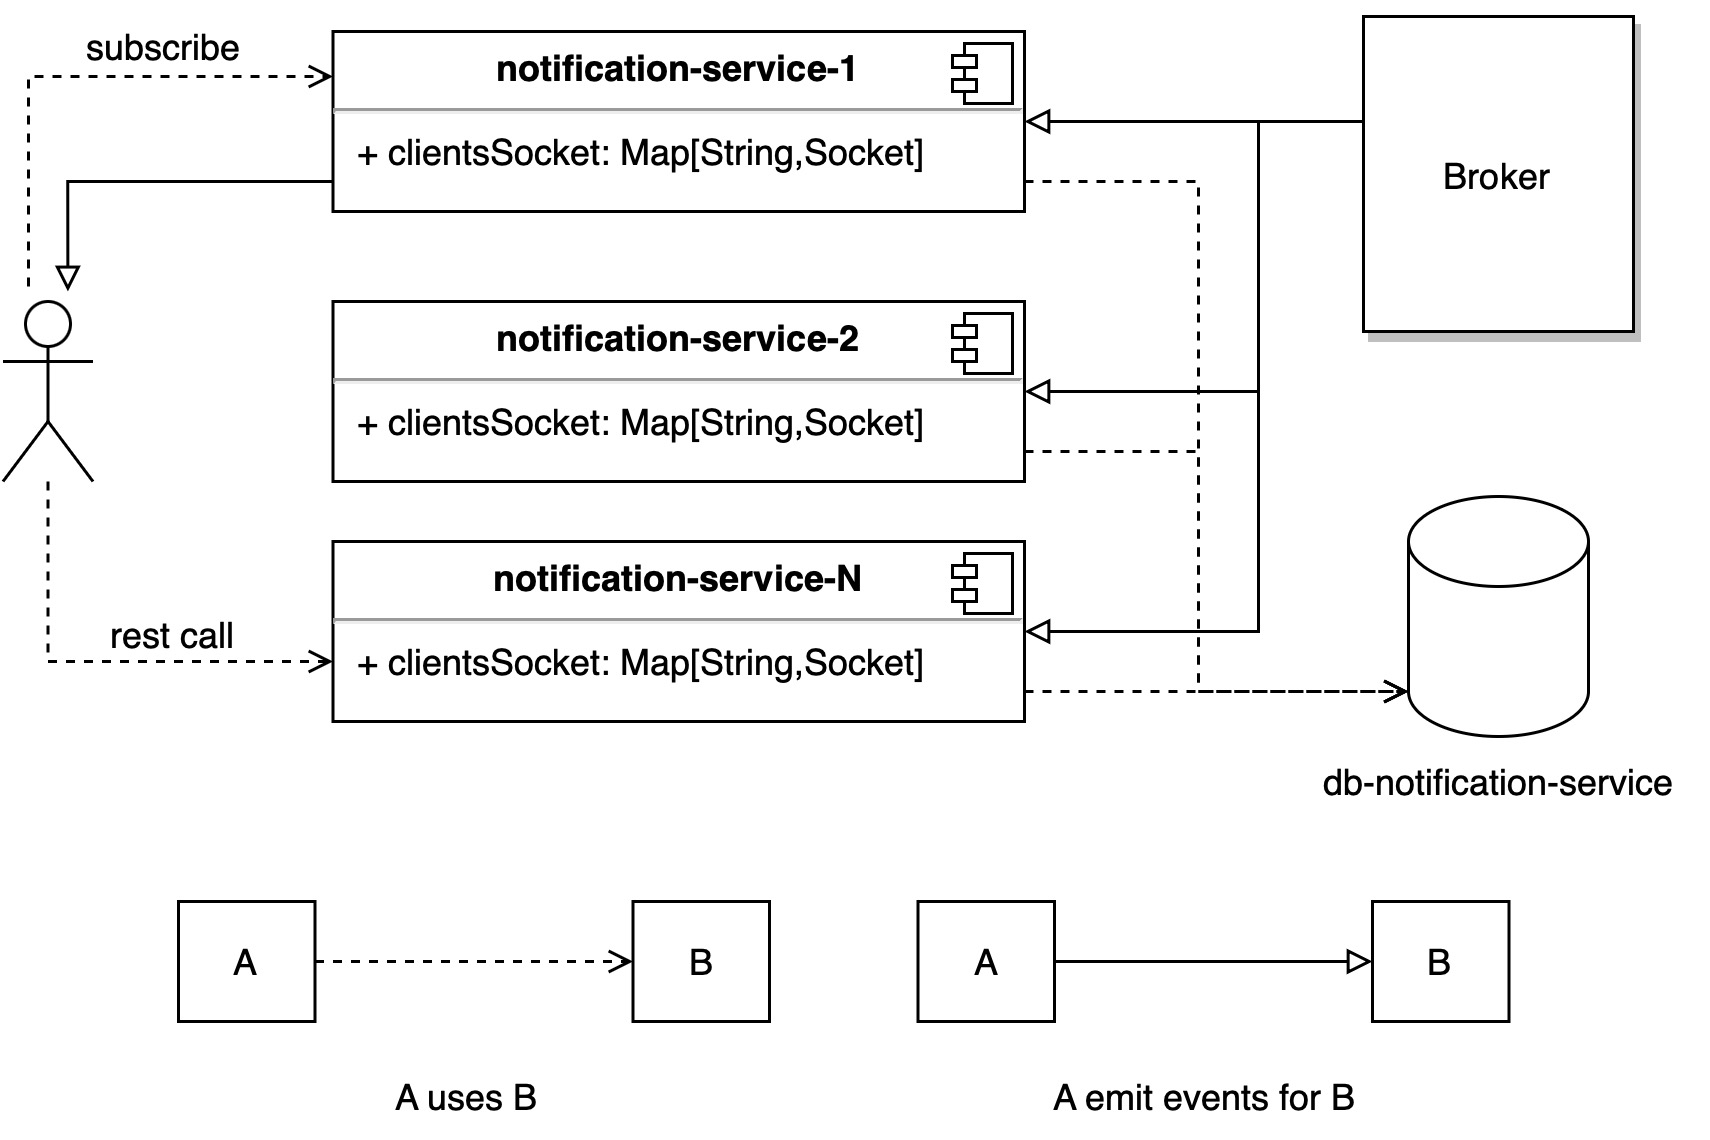
\includegraphics[width=\textwidth]{sections/04-implementation/img/notification-replication.jpg}
    \caption{Un utente crea una connessione persistente}
\end{figure}

%
%
%
\subsubsection{Socket.IO vs Server Sent Event}

Durante le fasi iniziali del progetto, al fine di inviare le notifiche dal microservizio verso il client, era stata adottato \emph{Server-Sent Events}\footnote{\url{https://developer.mozilla.org/en-US/docs/Web/API/Server-sent_events}}, una tecnologia di comunicazione monodirezionale, che permette di ricevere dati da un server che li invia.

Questo approccio è stato successivamente sostituito da Socket.IO perché il server non può gestire in modo responsivo la chiusura di una connessione da parte del client.

%
%
%
\subsection{WebRTC}

\emph{WebRTC}\footnote{\url{https://developer.mozilla.org/en-US/docs/Web/API/WebRTC_API}}, acronimo di “Web Real-Time Communication", è una tecnologia open-source che consente la comunicazione audio e video in tempo reale direttamente tra browser web senza richiedere plugin o software aggiuntivi.
%
È utilizzato per creare applicazioni di videoconferenza, chat video, streaming multimediale e altro.

Le principali caratteristiche di WebRTC includono:

\begin{enumerate}
    \item \textbf{Comunicazione peer-to-peer}: WebRTC consente ai browser di comunicare direttamente tra loro, evitando la necessità di server intermediari per la trasmissione di dati in tempo reale.

    \item \textbf{Supporto per audio e video}: WebRTC supporta la comunicazione audio e video in tempo reale, consentendo agli utenti di interagire tramite chat video o conferenze online.

    \item \textbf{Accesso ai dispositivi}: WebRTC consente l'accesso ai dispositivi hardware come telecamere e microfoni per abilitare la cattura audio e video.
\end{enumerate}

%
%
%
\subsubsection{Funzionamento}
Nel contesto di WebRTC, ci sono tre concetti chiave: \textbf{offer}, \textbf{answer}, e \textbf{ICE candidates}.

\begin{itemize}
    \item \textbf{Offer}:
    L'offerta è il punto di partenza per l'inizializzazione di una connessione WebRTC.

    Un peer (la parte che inizia la connessione) crea un'offerta che specifica le sue preferenze per la sessione di comunicazione, inclusi i codec supportati, i parametri di sicurezza, etc.
    L'offerta è creata utilizzando l'API \textit{createOffer().}

    \item \textbf{Answer}:
    L'answer è generata dal peer destinatario in risposta all'offerta ricevuta.
    %
    Il peer destinatario, dopo aver ricevuto l'offerta, crea una risposta che riflette le sue preferenze per la comunicazione.
    L'answer è creata utilizzando l'API \textit{createAnswer().}

    \item \textbf{ICE Candidates}:
    ICE (Interactive Connectivity Establishment) è un protocollo utilizzato per stabilire una connessione in presenza di reti complesse, come dietro firewall o NAT.
    I candidati ICE sono gli indirizzi IP e le porte su cui un peer può essere contattato.
    Durante il processo di offerta e risposta, i peer scambiano i loro candidati ICE utilizzando l'API \textit{onIceCandidate()}.
    Il processo di raccolta dei candidati ICE è noto come “ICE gathering".
\end{itemize}

In sintesi, il flusso tipico di inizializzazione di una connessione WebRTC coinvolge la creazione di un'offerta da parte del peer iniziatore, la trasmissione di questa offerta al peer destinatario, la creazione di una risposta da parte del peer destinatario e, infine, lo scambio di candidati ICE per stabilire una connessione diretta tra i due peer.
%
Questo processo è fondamentale per consentire la comunicazione bidirezionale in tempo reale tra browser senza passare attraverso un server intermedio.

%
%
%
\subsubsection{Sessione multimediale}
La gestione delle sessioni per le videochiamate WebRTC si basa su un modello che prevede l'utilizzo di sessioni individuali, ciascuna identificata da un unico ID e caratterizzata da un insieme di utenti consentiti (“allowed users") e dagli attuali partecipanti durante la chiamata in corso.
%
Ogni amicizia tra utenti è associata a una propria sessione, e lo stesso vale per i canali multimediali, i quali fanno riferimento a una sessione per agevolare le chiamate multimediali.

Le sessioni vengono distintamente gestite in base al contesto.
%
Nel caso delle amicizie, l'insieme di utenti consentiti è limitato esclusivamente ai due partecipanti dell'amicizia, garantendo una comunicazione privata tra i diretti interessati.
%
Invece, nei canali multimediali, l'insieme di utenti consentiti comprende tutti i partecipanti del server, consentendo così chiamate multimediali che coinvolgono più membri contemporaneamente.

Questo approccio alla gestione delle sessioni offre un controllo granulare sull'accesso alle videochiamate, garantendo che la comunicazione sia personalizzata in base al contesto delle relazioni tra gli utenti.
%
Inoltre, consente una scalabilità efficiente per le chiamate multimediali su larga scala, consentendo a tutti i partecipanti del server di partecipare alle conversazioni senza compromettere la sicurezza o la privacy delle comunicazioni one-to-one.

%
%
%
\subsubsection{Protocollo Signaling}

Di seguito il protocollo utilizzato per la procedura di signaling webrtc che permette lo scambio delle informazioni necessarie all instauramento delle connessioni p2p. 

\begin{figure}[H]
    \centering
    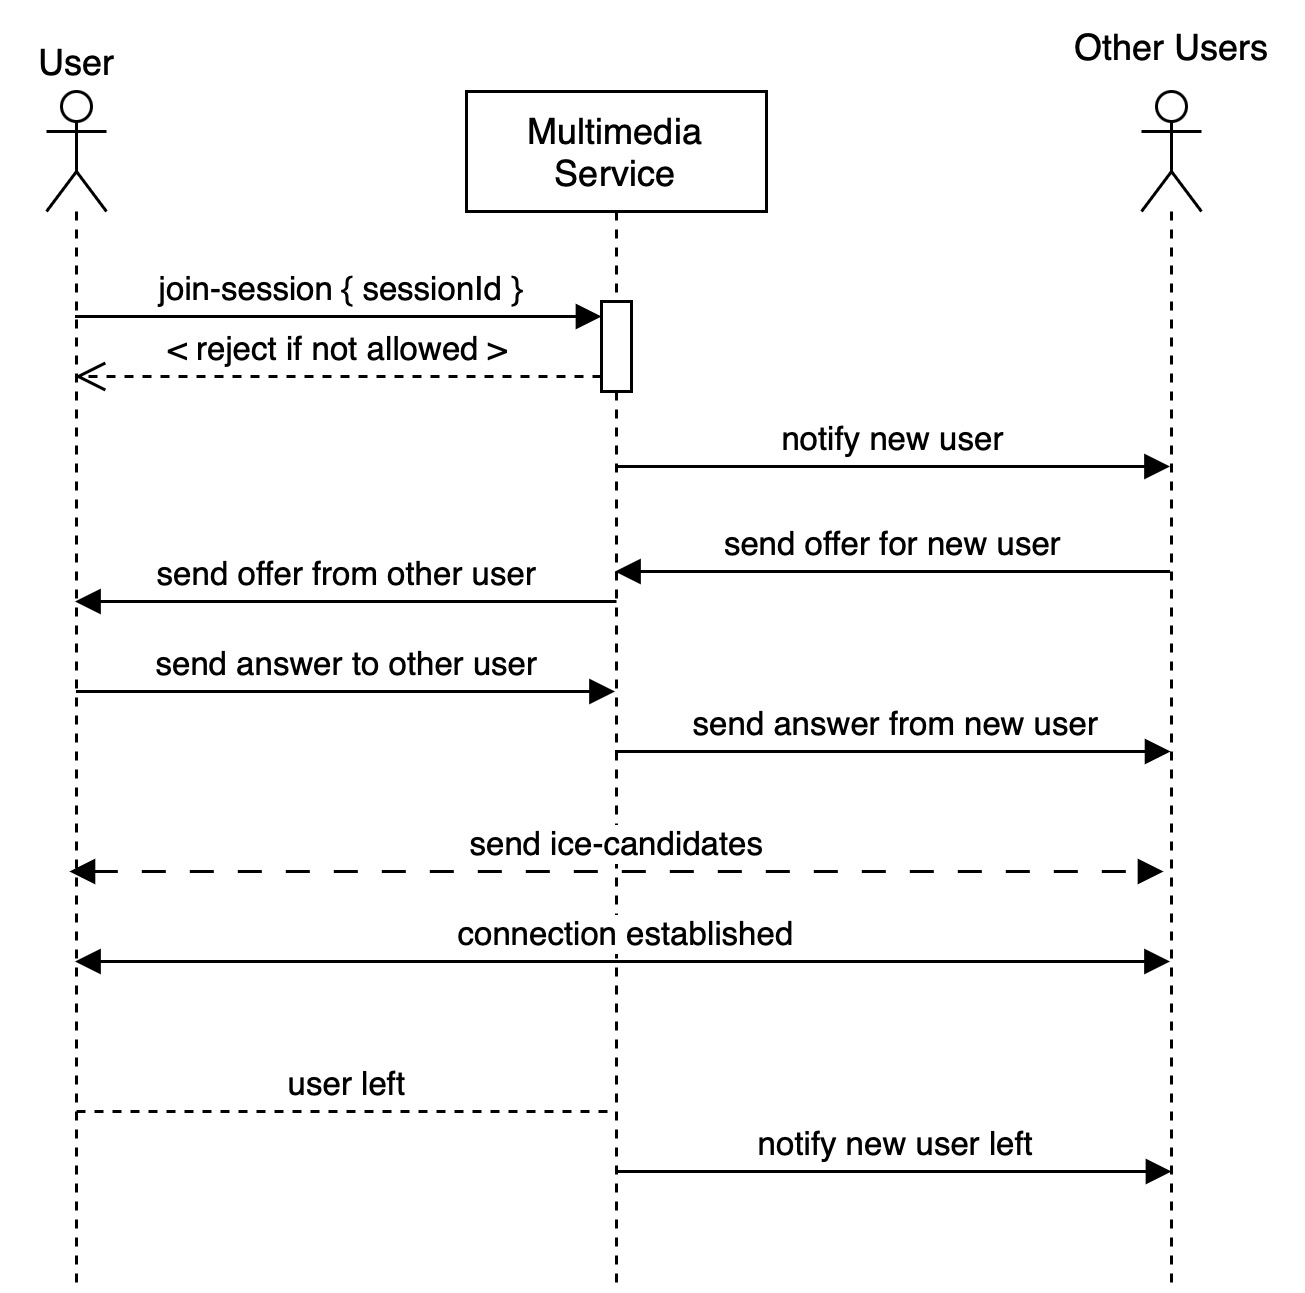
\includegraphics[width=0.9\textwidth]{sections/04-implementation/img/piperchat-Multimedia.jpg}
    % \caption{Protocollo signaling sessioni multimediali}
    \label{fig:piperchat-signaling}
\end{figure}

%
%
%
\subsubsection{Problema P2P e TURN}

Uno dei problemi principali che WebRTC deve affrontare è la presenza di dispositivi di rete con NAT (Network Address Translation) non compatibili, che possono complicare la creazione di connessioni dirette tra i partecipanti.

Il NAT consente a più dispositivi di condividere un singolo indirizzo IP pubblico, fornendo una forma di sicurezza e limitando la quantità di traffico Internet diretto verso dispositivi locali. Tuttavia, questo può creare problemi quando si tenta di stabilire connessioni dirette tramite WebRTC, in quanto alcuni NAT possono impedire il passaggio dei pacchetti dati necessari.

Per superare questo problema, WebRTC utilizza un concetto chiamato \textit{Traversal Using Relays around NAT (TURN)}. Un server TURN agisce come intermediario tra i partecipanti, aiutando a instradare i dati quando le connessioni dirette non sono possibili. Quando due peer non possono stabilire una connessione diretta a causa di NAT non compatibili, i dati vengono instradati attraverso il server TURN, consentendo comunque la comunicazione in tempo reale.

Per ovviare a questa problematica è stato quindi aggiunto al deploy anche un servizio adibito a funzionare da TURN in caso non sia possibile la connessione p2p.

%
%
%
\subsection{Autenticazione degli utenti}

Per gestire l'autenticazione degli utenti all'interno del nostro sistema, è stata adottata la tecnologia \textit{JSON Web Token (JWT)}.

%
%
%
\subsubsection{JWT}

JSON Web Token (JWT) è uno standard aperto (RFC 7519) che definisce un modo compatto per rappresentare informazioni tra due parti.
%
Queste informazioni possono essere verificate e fidate, poiché sono firmate digitalmente.

%
%
%
\paragraph{Struttura dei JWT}

Un JWT è costituito da tre parti separate da punti (.), che sono:

\begin{itemize}
    \item \textbf{Header:} Contiene il tipo di token (che è JWT) e l'algoritmo di firma utilizzato, ad esempio, HMAC SHA256 o RSA.
    
    \item \textbf{Payload:} Contiene le dichiarazioni, chiamate anche \textit{claim}, che rappresentano l'entità (solitamente l'utente) e le informazioni aggiuntive. %Esistono tre tipi di claim: registrati, pubblici e privati.
    
    \item \textbf{Signature:} Per ottenere la firma, si prende l'header codificato, il payload codificato, una chiave segreta, e si applica un algoritmo specifico. Questa firma viene aggiunta al token.
\end{itemize}

%
%
%
\paragraph{Funzionamento}

Quando un utente si autentica, riceve un JWT che può includere informazioni come l'identità e i diritti di accesso. Da quel momento in poi, il client invia il JWT con ogni richiesta successiva al server, che può verificare la firma del token per assicurarsi che sia valido. In questo modo, il server può fidarsi delle informazioni contenute nel JWT senza doverle verificare ad ogni richiesta.

%
%
%
\paragraph{Utilizzo}

Nel contesto di Piperchat, quando un utente si autentica con successo, il microservizio \texttt{Users} genera un JWT contenente nel payload le informazioni relative all'identità dell'utente. Questo JWT viene restituito al client, che lo utilizzerà nelle successive richieste per dimostrare la propria autenticità.

Inoltre, viene memorizzato nel database un token di refresh, che consente di ottenere nuovi token di accesso senza dover effettuare nuovamente l'accesso.

Quando il token di accesso scade, il client può richiedere un nuovo token di accesso al server utilizzando il token di refresh. Questo processo aiuta a mantenere un'esperienza utente fluida, riducendo al contempo il rischio di accessi non autorizzati.

%In sintesi, l'utilizzo di JSON Web Token all'interno di PiperChat offre un meccanismo robusto per l'autenticazione degli utenti, facilitando al contempo la gestione dei token sia lato client che lato server.

%
%
%
\subsection{Definizione delle API}

Per quanto riguarda la gestione delle api dei vari microservizi si è optato per avere una struttura che rappresentasse ogni endpoint, incapsulando sia i dati richiesti sia le possibili risposte.

A supporto di ciò è stato creato un modulo \textbf{api} che incapsula tutti gli endpoint del backend con le relativi informazioni.

Tale modulo viene sfruttato sia dal backend, per avere un typing migliore e un controllo di validazione dei parametri richiesti, che dal frontend per sapere già quali sono codice di risposta e tipologie di risposta per un determinato endpoint.

\begin{lstlisting}[style=typescript, caption={Definizione API}, label=lst:login:api]
export module LoginApi {

  export module Request {
    export type Body = {
      username: string
      password: string
    }
    export const Schema: RequestSchema = {
      Body: {
        username: 'string',
        password: 'string',
      },
    }
  }

  export module Responses {
    export class Success extends Response {
      statusCode = 200
      message = 'Logged in' as const
      jwt: string
    }
  }

  export module Errors {
    export class UsernameOrPasswordIncorrect extends ErrorResponse {
      statusCode = 401
      error = 'Username or password incorrect' as const
    }
  }
}
\end{lstlisting}

%
%
%
\subsection{Definizione degli Endpoint}

Una volta costruita la struttura rappresentante le singole API è stata creata l'utility \textbf{Route}, che a partire da un api permette di implementare l'endpoint aggiungendo il supporto automatico alla validazione dei dati in modo che se i dati in ingresso non dovessero essere corretti,  l'handler non venga notificato e venga restituito un messaggio di errore \textit{Bad Request}.
%
Inoltre permette e di dichiarare come reagire per ogni tipo di errore senza doverli controllare all'interno dell'handler.

Altra utilità offerta dalla classe è il typing dei parametri della richiesta basati sulle api specificate.

\begin{lstlisting}[style=typescript, caption={Definizione API}, label=lst:login:route]
export const LoginApiRoute = new Route<
  ...
>({
  method: 'post',
  path: '/login',
  schema: LoginApi.Request.Schema,
  handler: async (req, res) => {
    const token = await authController.login(req.body.username, req.body.password)
    res.sendResponse(new LoginApi.Responses.Success(token))
  },
  exceptions: [
    {
      exception: InvalidUsernameOrPassword,
      onException: (e, req, res) => {
        res.sendResponse(new UsernameOrPasswordIncorrect())
      },
    },
  ],
})
\end{lstlisting}

%
%
%
\subsection{Definizione dei Controller}

Per interfacciarsi con gli endpoint del backend sono quindi stati realizzati i \textbf{Controller} lato frontend, che incapsulano la gestione delle API fruttando il modulo opportuno per ottenere un typing delle richieste e delle risposte.

\begin{lstlisting}[style=typescript, caption={Definizione Controller}, label=lst:controller]
export class AuthControllerImpl extends AxiosController implements AuthController {
  async register(request: RegisterApi.Request.Type): Promise<RegisterApi.Response> {
    const body = request as RegisterApi.Request.Body
    return await this.post<RegisterApi.Response>('/auth/register', body)
  }

  async login(request: LoginApi.Request.Type): Promise<LoginApi.Response> {
    const body = request as LoginApi.Request.Body
    return await this.post<LoginApi.Response>('/auth/login', body)
  }

  async logout(): Promise<LogoutApi.Response> {
    return await this.post<LogoutApi.Response>('/auth/logout', {})
  }

  async refreshToken(): Promise<RefreshTokenApi.Response> {
    return await this.post<RefreshTokenApi.Response>(
        '/auth/refresh-token', {})
  }
}
\end{lstlisting}

%
%
%
\subsection{Monitoring}

Per monitorare lo stato dei servizi, è stato esposto un endpoint che restituisce un oggetto JSON contenente lo stato corrente e l'orario dell'ultimo aggiornamento.
%
Per garantire l'aggiornamento continuo del client rispetto a queste informazioni, si è optato per l'implementazione di un meccanismo di polling dal client al server.
%
Questa scelta consente al client di mantenere costantemente aggiornato lo stato dei servizi, anche nel caso in cui il server o i singoli microservizi diventino temporaneamente indisponibili.
%
In questo modo, il comportamento del client rimarrà invariato, assicurando una sincronizzazione continua con lo stato più recente dei servizi monitorati.
%
Inoltre, il microservizio di monitoraggio effettua anch'esso polling nei confronti degli altri microservizi per verificare se riceve risposta o meno.

\begin{lstlisting}[style=typescript, caption={Monitoring Polling - Client}, label=lst:ClientMonitoringPolling]
onMounted(async () => {
  await monitoringStore.refreshServicesStatus()
  setInterval(monitoringStore.refreshServicesStatus, 2000)
})
\end{lstlisting}

\subsection{Recap tecnologie utilizzate}

Di seguito un elenco di tutte le tecnologie utilizzate all'interno del progetto:

\subsubsection{Infrastruttura}
\begin{itemize}
    \item \textit{Docker} per il deploy dei container.
    \item \textit{Traefik} come Api-Gateway.
    \item \textit{RabbitMQ} come Broker.
\end{itemize}

\subsubsection{Microservizio}
\begin{itemize}
    \item \textit{NodeJS} come runtime environment.
    \item \textit{Typescript} come linguaggio di sviluppo.
    \item \textit{Express} per lo sviluppo dei Webserver.
    \item \textit{MongoDB} come database.
    \item \textit{Mongoose} come libreria per l'utilizzo di database Mongo.
    \item \textit{JWT} per la gestione dell'autenticazione.
    \item \textit{Jest} come framework di Unit testing.
\end{itemize}

\subsubsection{Frontend}
\begin{itemize}
    \item \textit{Vue.js} per lo sviluppo della Single Page Application.
    \item \textit{Pinia} per la gestione degli store.
    \item \textit{Quasar} per la realizzazione dei componenti grafici.
\end{itemize}

\subsubsection{Comunicazione}
\begin{itemize}
    \item \textit{Axios} per la gestione di richieste HTTP.
    \item \textit{Socket.io} per le comunicazioni real-time.
    \item \textit{WebRTC} per le videochiamate.
\end{itemize}

\subsubsection{Documentazione}
\begin{itemize}
    \item \textit{Swagger} per la documentazione delle API.
    \item \textit{AsyncAPI} per la documentazione dei messaggi infra-servizio.
\end{itemize}